\section{Results}
The parameters used in the simulation of a spiral galaxy are shown in \autoref{tab:galaxy-parameters}.
\begin{table}[htp]
    \centering
    \begin{tabular}{|l|c|}
        \hline
        \textbf{Parameter}      & \textbf{Value}           \\
        \hline
        Central bulge radius    & 3 kpc                    \\
        Central bulge mass      & $60 \times 10^9 M_\odot$ \\
        Disk radius             & 15 kpc                   \\
        Disk mass               & $15 \times 10^9 M_\odot$ \\
        Disk thickness          & 0.3 kpc                  \\
        Disk density profile    & Uniformly decreasing     \\
        Mass assignment scheme  & TSC                      \\
        Finite difference       & Two-point                \\
        Time integration method & Leapfrog                 \\
        \hline
    \end{tabular}
    \caption{Galaxy model parameters used in the simulation.}
    \label{tab:galaxy-parameters}
\end{table}

\subsection{particle-mesh method}
In the PM method $N=50,000$ particles were used.
Cell size $H$ and time-step length were set to $60/64=0.9375$ kpc, and 1 Myr respectively.
The evolution of the system over 200 Myrs is shown in \autoref{fig:spiral-galaxy-evolution-pm}.

\begin{figure}[htp]
    \centering
    \begin{subfigure}[b]{0.45\textwidth}
        \centering
        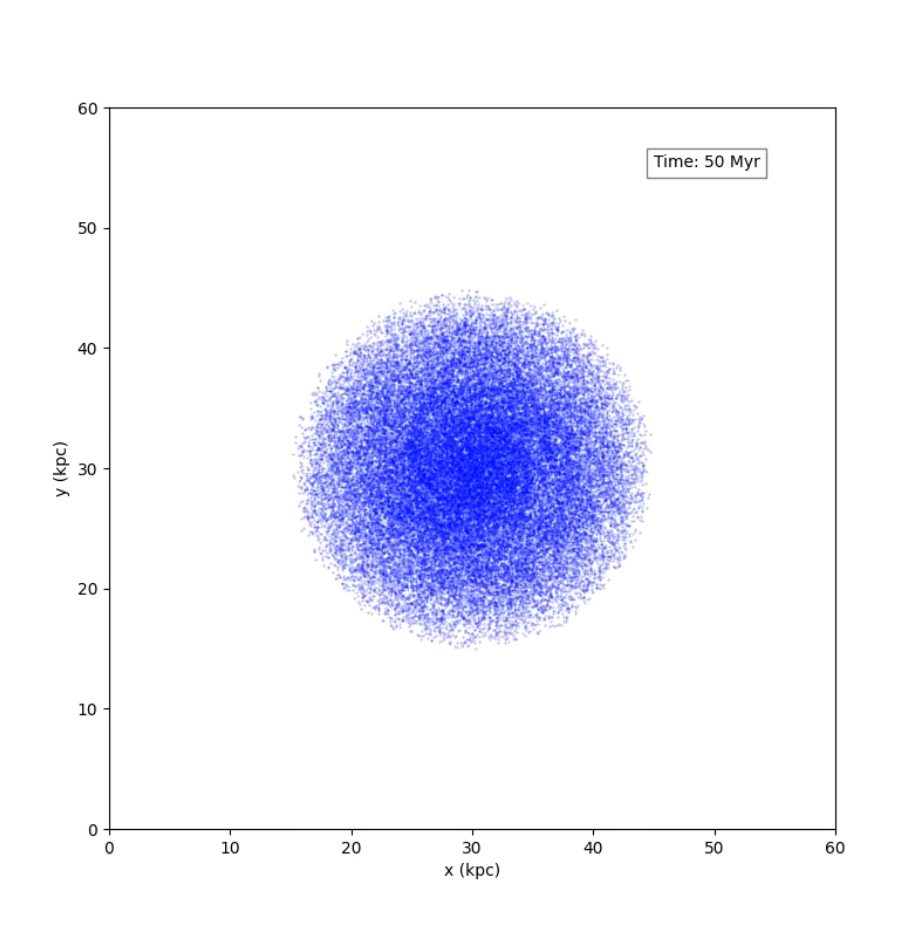
\includegraphics[width=\textwidth]{img/pm/50myr.png}
        \caption{$t=50\,\text{Myr}$}
        \label{fig:spiral-galaxy-evolution-pm-sub1}
    \end{subfigure}
    \hfill
    \begin{subfigure}[b]{0.45\textwidth}
        \centering
        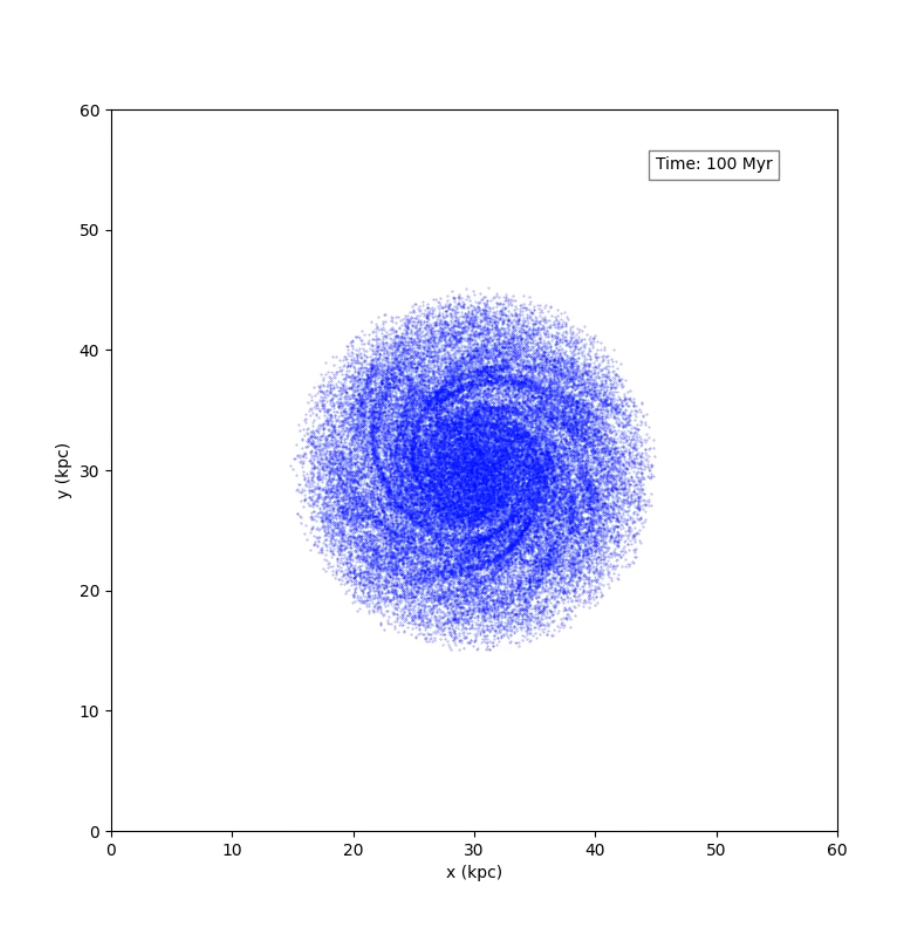
\includegraphics[width=\textwidth]{img/pm/100myr.png}
        \caption{$t=100\,\text{Myr}$}
        \label{fig:spiral-galaxy-evolution-pm-sub2}
    \end{subfigure}

    \vspace{0.5cm}

    \begin{subfigure}[b]{0.45\textwidth}
        \centering
        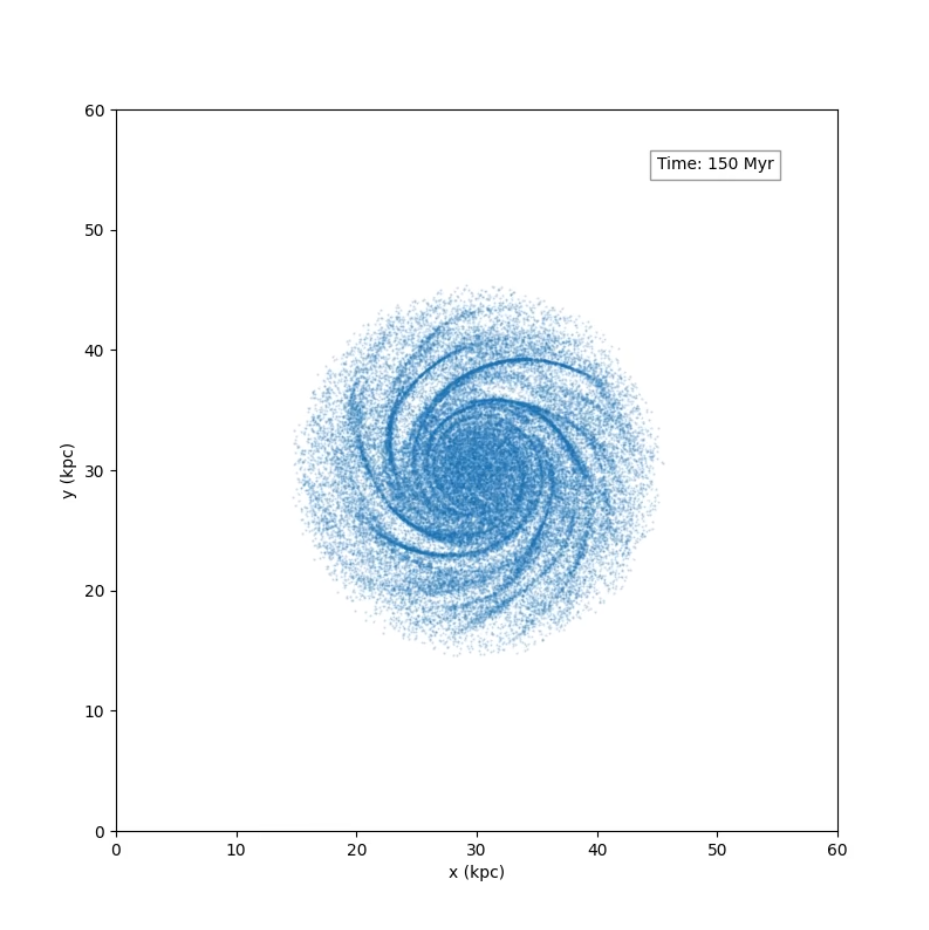
\includegraphics[width=\textwidth]{img/pm/150myr.png}
        \caption{$t=150\,\text{Myr}$}
        \label{fig:spiral-galaxy-evolution-pm-sub3}
    \end{subfigure}
    \hfill
    \begin{subfigure}[b]{0.45\textwidth}
        \centering
        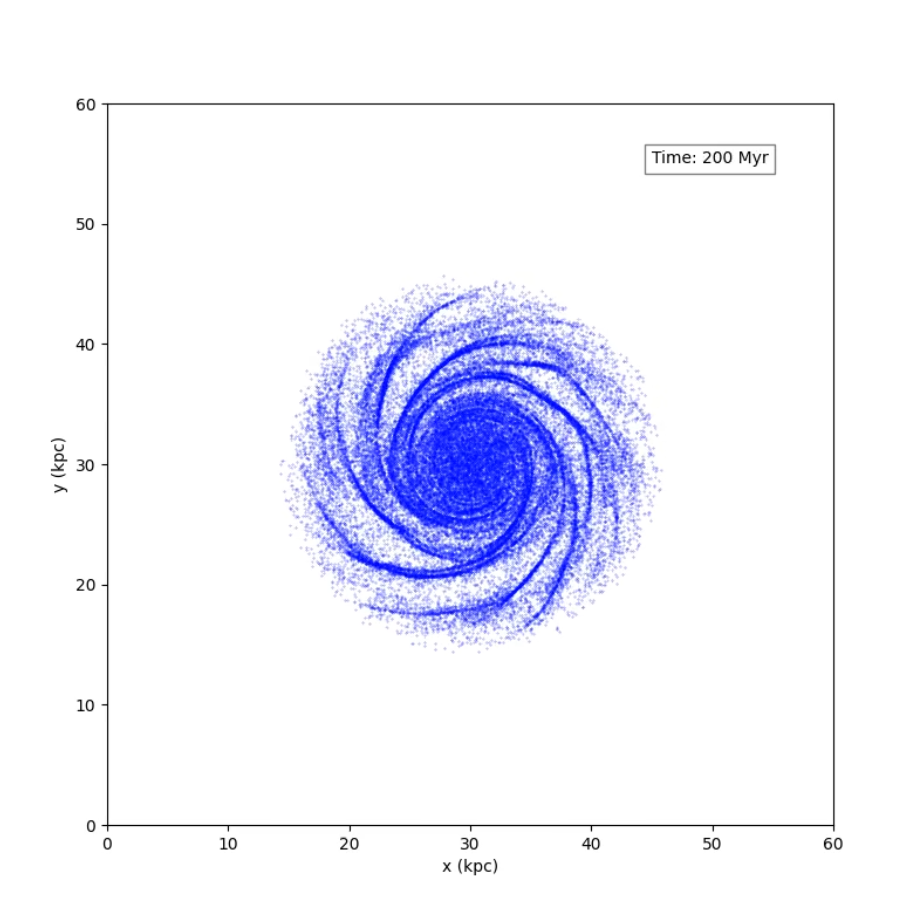
\includegraphics[width=\textwidth]{img/pm/200myr.png}
        \caption{$t=200\,\text{Myr}$}
        \label{fig:spiral-galaxy-evolution-pm-sub4}
    \end{subfigure}

    \caption{Evolution of a spiral galaxy as predicted by the PM method.}
    \label{fig:spiral-galaxy-evolution-pm}
\end{figure}

During the simulation, total energy $E = KE + PE$, angular momentum $\mathbf{l}$ and the $z$-component of the momentum vector $\mathbf{p}$ should stay constant.
The $x$- and $y$-components of momentum change due to presence of external gravitational field (central bulge).
We can verify if this variation satisfies the expected relation
\begin{equation}\label{eq:expected-momentum-change}
    \dot{\mathbf{p}} = \mathbf{F}^\text{ext}
\end{equation}
by fining the initial total momentum $\mathbf{p}(t = 0)$ and incrementing the value of $\mathbf{p}$ in each time-step by $\mathbf{F}^{ext}DT$.
\begin{figure}[htp]
    \centering
    \begin{subfigure}[b]{0.45\textwidth}
        \centering
        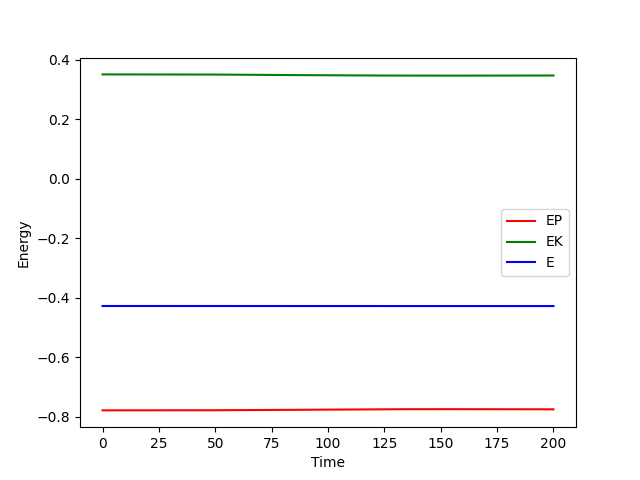
\includegraphics[width=\textwidth]{img/pm/energy.png}
        \caption{Energy}
        \label{fig:physical-quantities-pm-sub1}
    \end{subfigure}
    \hfill
    \begin{subfigure}[b]{0.45\textwidth}
        \centering
        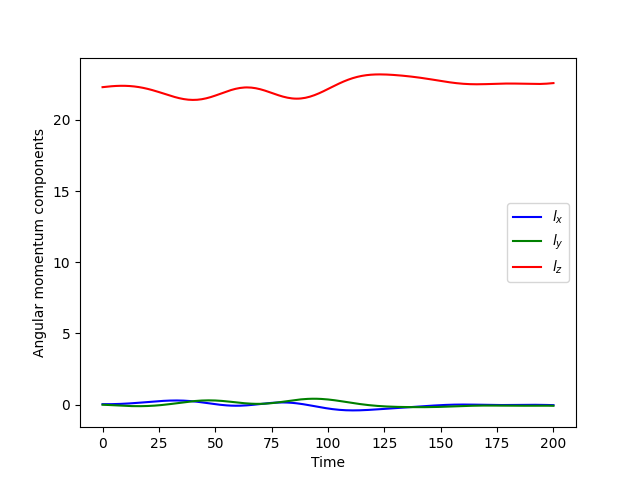
\includegraphics[width=\textwidth]{img/pm/angular-momentum.png}
        \caption{Angular momentum}
        \label{fig:physical-quantities-pm-sub2}
    \end{subfigure}

    \vspace{0.5cm}

    \begin{subfigure}[b]{0.45\textwidth}
        \centering
        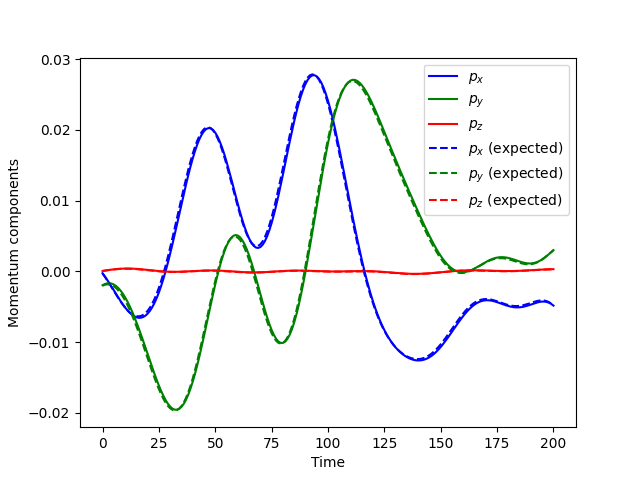
\includegraphics[width=\textwidth]{img/pm/momentum.png}
        \caption{Momentum; broken lines represent the expected momentum following \autoref{eq:expected-momentum-change}}
        \label{fig:physical-quantities-pm-sub3}
    \end{subfigure}

    \caption{Fundamental physical quantities describing the system over time in the PM simulation.
        Time is in Myr and the quantities are expressed in units consistent with \autoref{tab:galaxy-parameters}}
    \label{fig:physical-quantities-pm}
\end{figure}

\subsection{particle-particle particle-mesh method}
The \PThreeM{} based simulation uses the same parameters as the PM method.
One extra free parameter is the \textit{softening length} $\epsilon$ which modifies the universal law of gravitation so that division by zero can be avoided, i.e. the modified law is
\begin{equation*}
    F_\text{soft}(r) = \frac{G m_i m_j}{r_{ij}^2 + \epsilon^2}.
\end{equation*}
In the simulation, $\epsilon$ was set arbitrarily to $1.5$ kpc.
The evolution of the system is depicted in \autoref{fig:spiral-galaxy-evolution-p3m}.
\begin{figure}[htp]
    \centering
    \begin{subfigure}[b]{0.45\textwidth}
        \centering
        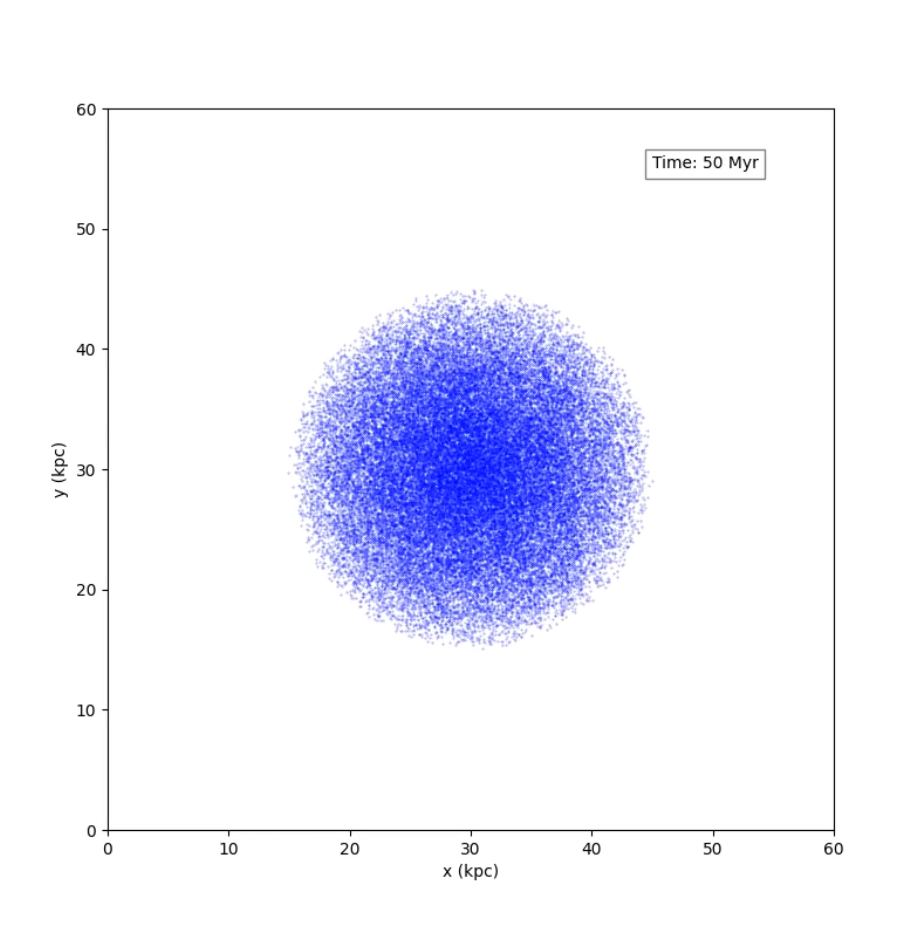
\includegraphics[width=\textwidth]{img/p3m/50myr.png}
        \caption{$t=50\,\text{Myr}$}
        \label{fig:spiral-galaxy-evolution-p3m-sub1}
    \end{subfigure}
    \hfill
    \begin{subfigure}[b]{0.45\textwidth}
        \centering
        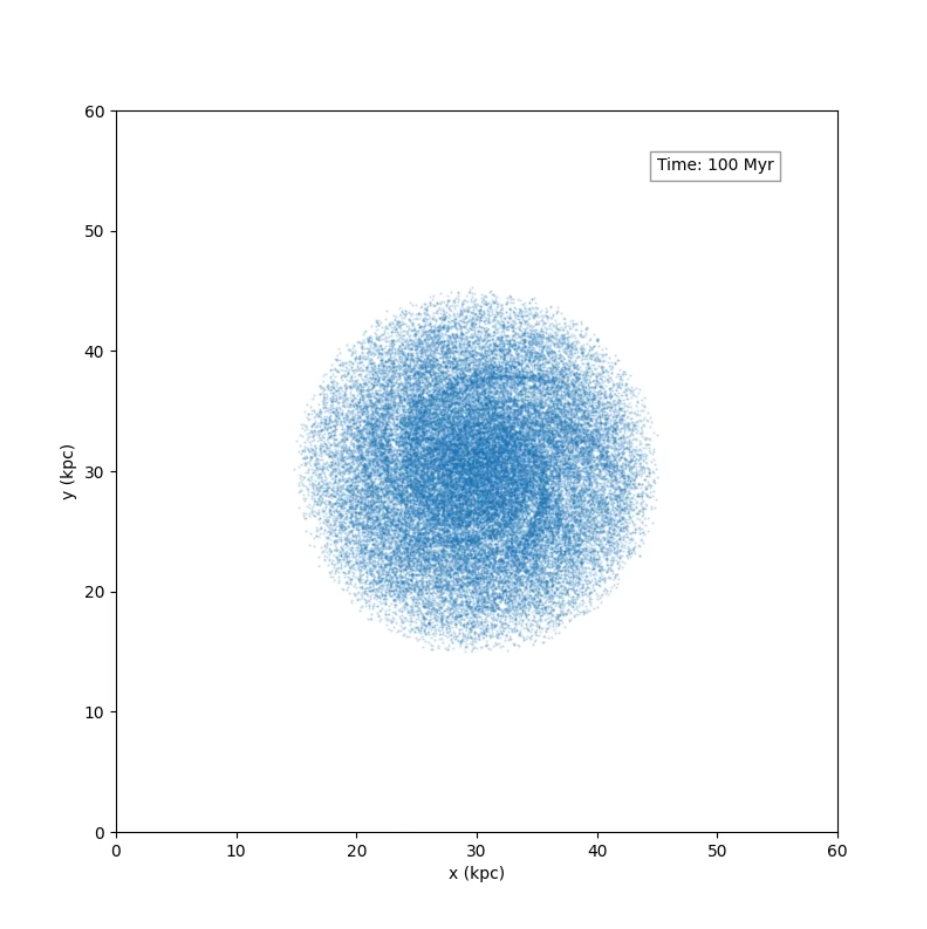
\includegraphics[width=\textwidth]{img/p3m/100myr.png}
        \caption{$t=100\,\text{Myr}$}
        \label{fig:spiral-galaxy-evolution-p3m-sub2}
    \end{subfigure}

    \vspace{0.5cm}

    \begin{subfigure}[b]{0.45\textwidth}
        \centering
        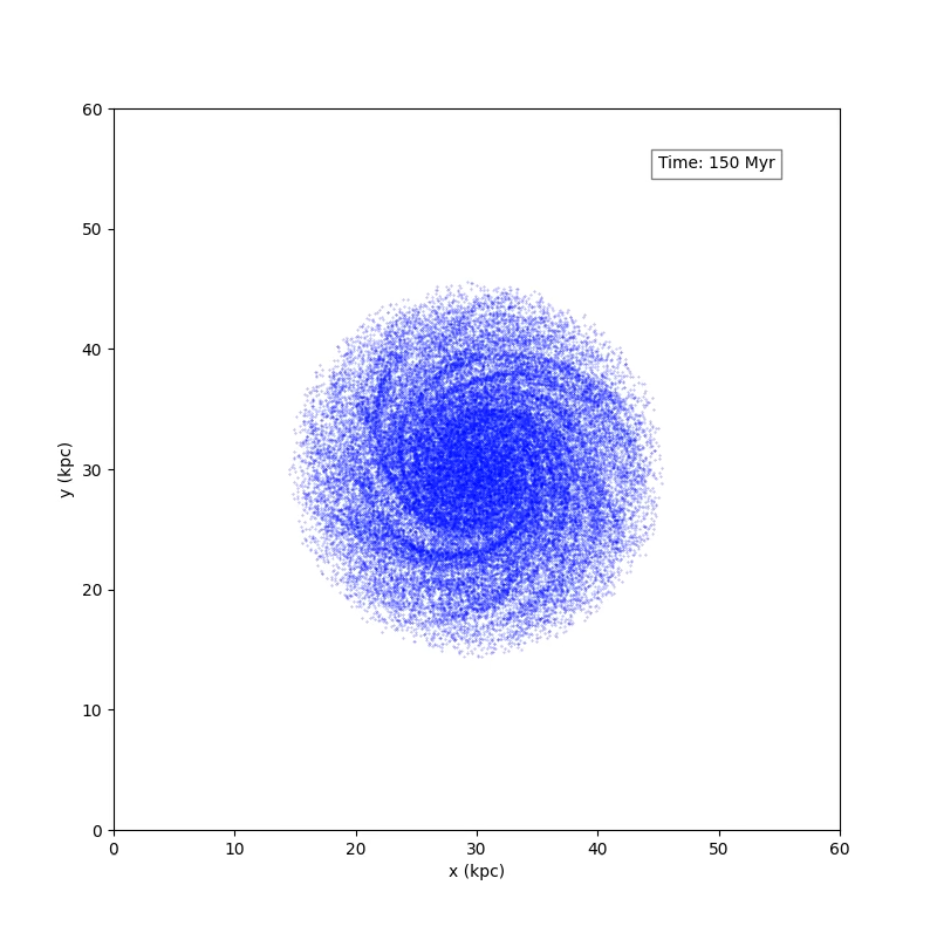
\includegraphics[width=\textwidth]{img/p3m/150myr.png}
        \caption{$t=150\,\text{Myr}$}
        \label{fig:spiral-galaxy-evolution-p3m-sub3}
    \end{subfigure}
    \hfill
    \begin{subfigure}[b]{0.45\textwidth}
        \centering
        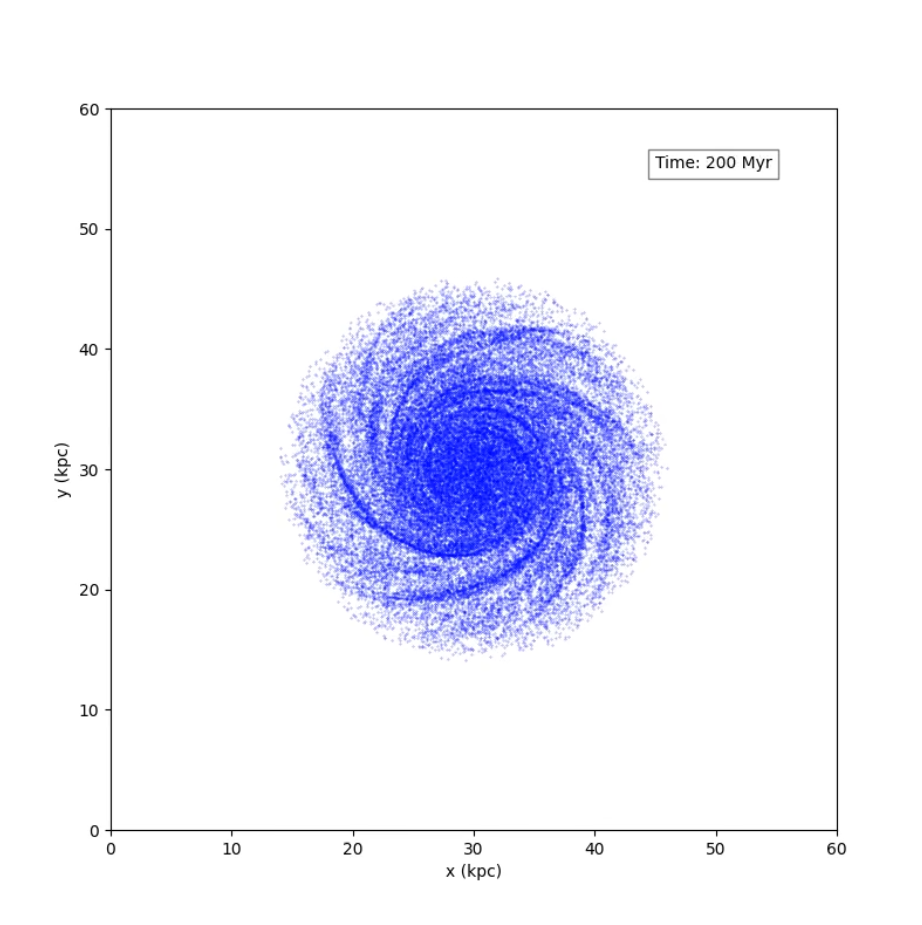
\includegraphics[width=\textwidth]{img/p3m/200myr.png}
        \caption{$t=200\,\text{Myr}$}
        \label{fig:spiral-galaxy-evolution-p3m-sub4}
    \end{subfigure}

    \caption{Evolution of a spiral galaxy as predicted by the \PThreeM{} method.}
    \label{fig:spiral-galaxy-evolution-p3m}
\end{figure}
Graphs of energy, angular momentum components, and momentum components vs. time are shown in \autoref{fig:physical-quantities-p3m}.
\begin{figure}[htp]
    \centering
    \begin{subfigure}[b]{0.45\textwidth}
        \centering
        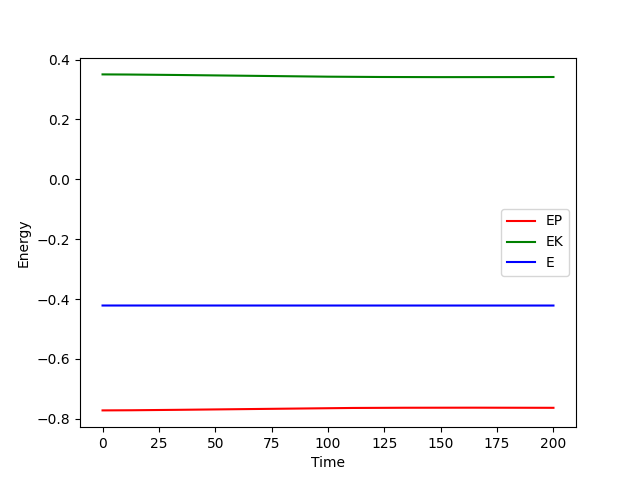
\includegraphics[width=\textwidth]{img/p3m/energy.png}
        \caption{Energy}
        \label{fig:physical-quantities-p3m-sub1}
    \end{subfigure}
    \hfill
    \begin{subfigure}[b]{0.45\textwidth}
        \centering
        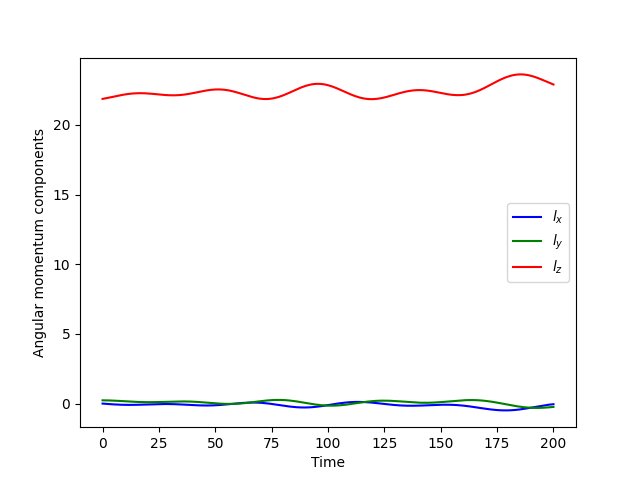
\includegraphics[width=\textwidth]{img/p3m/angular-momentum.png}
        \caption{Angular momentum}
        \label{fig:physical-quantities-p3m-sub2}
    \end{subfigure}

    \vspace{0.5cm}

    \begin{subfigure}[b]{0.45\textwidth}
        \centering
        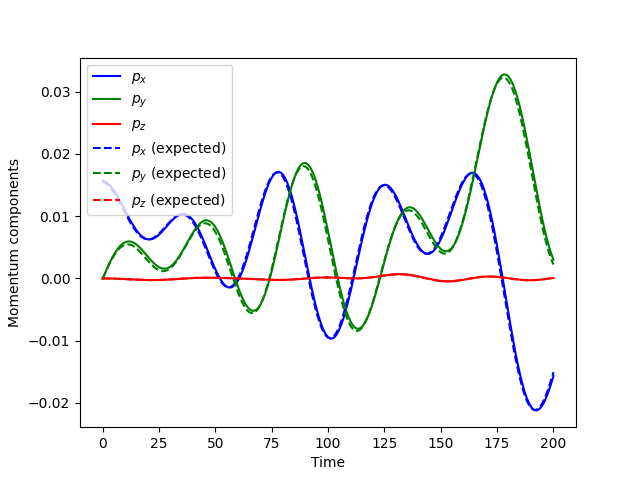
\includegraphics[width=\textwidth]{img/p3m/momentum.png}
        \caption{Momentum; broken lines represent the expected momentum following \autoref{eq:expected-momentum-change}}
        \label{fig:physical-quantities-p3m-sub3}
    \end{subfigure}

    \caption{Fundamental physical quantities describing the system over time in the \PThreeM{} simulation.
        Time is in Myr and the quantities are expressed in units consistent with \autoref{tab:galaxy-parameters}}
    \label{fig:physical-quantities-p3m}
\end{figure}